\documentclass[11pt, a4paper, USenglish]{article}

\usepackage{kyblab}

\begin{document}

% Contents
\title{TTK4145 Notes}
\author{Mikkel Tiller}
\date{}
\maketitle
\todo[inline, caption={}]{
TODO:
\begin{enumerate}
    \item Ada, exercises 7 and 8
    \item Modeling of concurrent programs, FSP
    \item Deadlocks
    \item The Little Book of Semaphores
    \item Scheduling, time-lines, priority ceiling protocols
    \item Transactions and atomic actions
\end{enumerate}
}
% \tableofcontents
\newpage
\part{Code quality}
Ultimate SW quality metric: \textbf{maintainability}. 
\section{Modules}
\begin{itemize}
    \item You should be able to use modules without knowledge of its internals.
    \item You should be able to maintain a module without knowledge of the rest of the system.
    \item Composition: Easy to build supermodules from submodules.
    \item Coupling: Weak coupling between modules.
    \item Cohesion: The parts of a module should be well connected. 
\end{itemize}
\newpage
\part{Fault tolerance}
Four sources of faults in embedded systems:
\begin{enumerate}
    \item Inadequate specification, i.e. misunderstanding the interactions between the program and environment.
    \item Design errors in software components. We typically don't know the consequences of these.
    \item Failure of hardware components. More predictable than the one above.
    \item Interference in the supporting communication subsystem.
\end{enumerate}

\section{Reliability, failure and faults}
\textbf{Reliability} is a measure of how well a system conforms to the specification of its behavior. \emph{Response times} are an important part of the specification. \textbf{Failure} is when a system deviates from the specification. Highly reliable $\iff$ low failure rate.

The above definitions are concerned with the systems behaviour (external appearance). Failure stems from internal errors, whose algorithmic or mechanical causes are called \textbf{faults}. This motivates the following definition of a faulty component: A faulty component is one that under certain circumstances, during the lifetime of the system, results in an error.

An external state that is not in the specification is regarded as a failure, and an internal state that that is not specified is called an error. A fault is \textbf{active} when it produces an error, otherwise it is \textbf{dormant}. The error propagates through the system, and manifests itself as part of the external behavior.

A failure in one (sub)system can cause faults in other systems, as the following chain of events illustrates:\\
Fault $\xrightarrow{\text{activation}}$ Error $\xrightarrow{\text{propagation}}$ Failure $\xrightarrow{\text{causation}}$ Fault\\

With regard to time, there are three kinds of faults:
\begin{enumerate}
    \item \textbf{Transient faults} occur at some point in time, then disappear at some later point in time. E.g. HW response to external electromagnetic field, fault disappears when the field disappears. Common kind of fault in communication systems.
    \item \textbf{Permanent faults} start at a particular time, then remain in the system until they are fixed. E.g. SW design error.
    \item \textbf{Intermittent faults} are transient faults that occur from time to time, common with e.g. heat sensitive HW.
\end{enumerate}
\textbf{Bugs} are software faults, and originally there were two kinds:
\begin{itemize}
    \item \textbf{Bohrbugs} are reproducible and identifiable, can be removed during testing or with design diversity techniques.
    \item \textbf{Heisenbugs} are only active under certain rare circumstances, and often disappear when investigated. An example is code shared between concurrent tasks that is not properly synchronized. Heisenbugs can result from software ageing, e.g. not freeing allocated memory, and exhausting the available memory after a long time. Restarting the system clears this bug.
\end{itemize}

\section{Failure modes}
A system provides services, and its failure modes can be classified according to their impact on these services. Two general classes:
\begin{itemize}
    \item \textbf{Value failure} - Error in the value associated with service. Can be the result of a data conversion, e.g. 64-bit to 8-bit.
    \item \textbf{Time failure} - Service not delivered at the correct time.
\end{itemize}
Combinations of the two are called \emph{arbitrary} failures. Time failures can result in the service being delivered:
\begin{itemize}
    \item too early
    \item too late (performance error)
    \item infinitely late (omission failure) 
\end{itemize}
How can a system fail?
\begin{enumerate}
    \item Fail uncontrolled - arbitrary errors
    \item Fail late - delivers service too late in the time domain
    \item Fail silent - ommision failure
    \item Fail stop - same as above, but permits other systems to detect that it has failed silently
    \item Fail controlled - fails in a specified controlled manner
    \item Fail never - self explanatory
\end{enumerate}

\section{Fault prevention and fault tolerance}
\textbf{Fault prevention} aims to eliminate any and all faults before the system goes into operation, whilst \textbf{fault tolerance} enables the system to continue functioning even in the presence of faults. Both approaches attempt to give the system well-defined failure modes.

\subsection{Fault prevention}
Two steps; fault avoidance and fault removal. Fault avoidance consists of:
\begin{itemize}
    \item Acquiring reliable hardware and protecting it against interference.
    \item Rigorous specification of requirements, design based on e.g. UML (avsky).
    \item Use languages with data abstraction and modularity, like Ada and Java.
\end{itemize}
Fault removal consists of removing causes of errors, mainly by systems tests. However, testing can never remove all potential faults:
\begin{itemize}
    \item A test can only show the presence of faults, not their absence.
    \item It might be impossible to test under realistic conditions.
    \item Errors from the requirement analysis might not become visible until the system is in operation.
\end{itemize}
Any system will fail eventually (HW or SW), and for real-time systems we need fault tolerance.

\subsection{Fault tolerance}
Three levels of fault tolerance:
\begin{enumerate}
    \item \textbf{Full fault tolerance} - operation continues without significant loss of performance, but only for a limited time.
    \item \textbf{Fail soft} - operation continues, but a partial degradation in performance is accepted until recovery or repair.
    \item \textbf{Fail safe} - the system's integrity is maintained, but a temporary halt in operation is accepted. I.e. the system is shut down in a safe state. 
\end{enumerate}
Back in the day fault-tolerant design was based on three assumptions:
\begin{enumerate}
    \item Algorithms are correctly designed.
    \item All failure modes are known.
    \item All possible interactions with the environment are known.
\end{enumerate}
This is not realistic today, with multi-core processors and such, hence both anticipated and unanticipated errors must be accounted for.

\subsection{Redundancy}
\textbf{Protective redundancy} introduces components that detects and recovers the systems from faults, but are unnecessary for normal operation. When designing a fault-tolerant system, the goal is to minimize redundancy while maximizing reliability, subject to constraints on cost, size and power consumption. The redundant components can (and will) increase complexity, and it is useful to separate them from the rest of the system. 

We separate between static and dynamic redundancy, both for hardware and software. First, let's have a look at hardware redundancy:
\begin{itemize}
    \item \textbf{Static redundancy} (or masking) is based on redundant components ``hiding'' faults. An example is Triple Modular Redundancy (TMR), where a majority voting circuit is used. The output of three identical components are compared, and if one differs from the others, its output is masked out. It is assumed that faults are transient.
    \item \textbf{Dynamic redundancy} is an error-detection facility within a component, making it possible for that component to indicate if its output is in error. Note that the component does not hide or fix the error, that must be done by some other part of the system. Examples are checksums (see parity byte section on Wikipedia for very simple example) and parity bits.
\end{itemize}

For fault tolerance with regards to software design, we have \emph{N-version programming} which works like masking, and \emph{error detection and recovery}. The latter is dynamic redundancy in the sense that recovery is only brought into action once an error has occured.

\section{N-version programming}
From one initial specification, N independent programs are created. In operation, they run concurrently, and their outputs are compared by a driver process. The ``correct'' result is determined by majority of vote, like with masking. Challenges concerning N-version programming are:
\begin{itemize}
    \item \textbf{Initial specification} - It is close to impossible to produce unambiguous specifications.
    \item A complex part of the specification can potentially induce faults for all the N independent developer teams.
    \item Budget concerns, N-versions are N times more expensive than one.
    \item \textbf{Granularity} - How often results are compared affects overhead in one direction, and fault tolerance in the other.
    \item \textbf{Inexact voting} - Results may not agree exactly, even when no fault has occured. This is a consequence of \emph{finite-precision} arithmetic and the possibility of multiple correct solutions (a quadratic eq. being a simple example). One solution is to regard values inside a range of $\Theta$ to be equal, but then the problem arises once again for values close to the boundaries of the range.
\end{itemize}

\section{Software dynamic redundancy}
Statically redundant components operate whether or not an error has occured. With dynamic redundancy, however, the redundant components are only put into play when an error occurs. There are four phases to dynamic redundancy in software:
\begin{enumerate}
    \item \textbf{Error detection}
    \item \textbf{Error diagnosis} - There is a delay between a fault becoming active and error detection, the propagation of erroneous information in the system is assessed.
    \item \textbf{Error recovery} - Transform the corrupted system into a state where it can continue operation.
    \item \textbf{Fault treatment} - Maintenance must be performed to correct the underlying fault responsible for the error.
\end{enumerate}

\subsection{Error detection}\label{sec:error_detection}
There are two classes:
\begin{itemize}
    \item \textbf{Environmental detection} - Detection by hardware (e.g. overflow error) or run-time support system (e.g. out of bounds error for array).
    \item \textbf{Application detection}
    \begin{itemize}
        \item \textbf{Replication checks} - Check if results are equal.
        \item \textbf{Timing checks} - Can be a \emph{wtachdog timer} that has to be reset with a given frequency, or detection of missed deadlines by the scheduling system.
        \item \textbf{Reversal checks} - Compute the input from the output, and compare with the actual input.
        \item \textbf{Coding checks} - E.g. checksum
        \item \textbf{Reasonableness checks} - \texttt{assert()}-function
        \item \textbf{Structural checks} - E.g. count number of elements in list to confirm integrity.
        \item \textbf{Dynamic reasonableness checks} - Error assumed if new output is too different from previous value.
    \end{itemize}
\end{itemize}

\subsection{Error diagnosis}
Software designers aim to minimize the damage caused by a faulty component, this is called \emph{firewalling}. Two techniques are: 
\begin{itemize}
    \item \textbf{Modular decomposition} - Modules only communicate through well-defined interfaces, internal details are hidden. Provides a static structure.
    \item \textbf{Atomic actions} are indivisible, and appear to happen instantaneously for the rest of the system. Often called \textbf{transactions} or atomic transactions. They are used to move the system from one consistent state to another, and limit the flow of information between components/modules.
    \item There are also \textbf{protection mechanisms} which may stop a process from accessing a resource based on its access permissions.
\end{itemize}

\subsection{Error recovery}
There are two approaches; \textbf{forward} and \textbf{backward} error recovery.

Forward error recovery tries to continue from an erroneous state by finding a new consistent (but probably sub-optimal) state.  An example is Hamming codes (haven't read about them). Useful if the error related to the previous state may happen many times in a row, and one cannot afford to return to that state.

Backward error recovery restores the system to a previous safe state, a \textbf{recovery point}, and executes a different code block than the one that lead to an error. The new code should have the same functionalty, but use a different algorithm. Setting up a recovery point is called \textbf{checkpointing}.

Backward recovery can be used to recover from unanticipated faults (very good), but cannot undo effects the fault had on the environment (e.g. launching a missile). Furthermore, it may be costly in a real-time sense to save state from time-varying sensor data.

State restoration with concurrent processes is not necessarily simple, as is seen from the \textbf{domino effect}. Let us say we have two processes, say $P_1$ and $P_2$ that communicate, synchronize and set up recovery points. If $P_1$ detects an error at time $T_e$, it will roll back to its previous safe state. But what if there was communication between $P_1$ and $P_2$ between that state and $T_e$? Then $P_2$ must also roll back to its previous state, and there might have been some communication in between there as well. This might continue until both processes are back to square one, and is called the \emph{domino effect}. 

The probability of the domino effect increases with the number of concurrent processes. A \textbf{recovery line}, a consisent set of recovery points, is required to avoid the effect.

\section{Recovery blocks}
\Cref{fig:recovery_block} illustrates a recovery block.
\begin{figure}[]
    \centering
    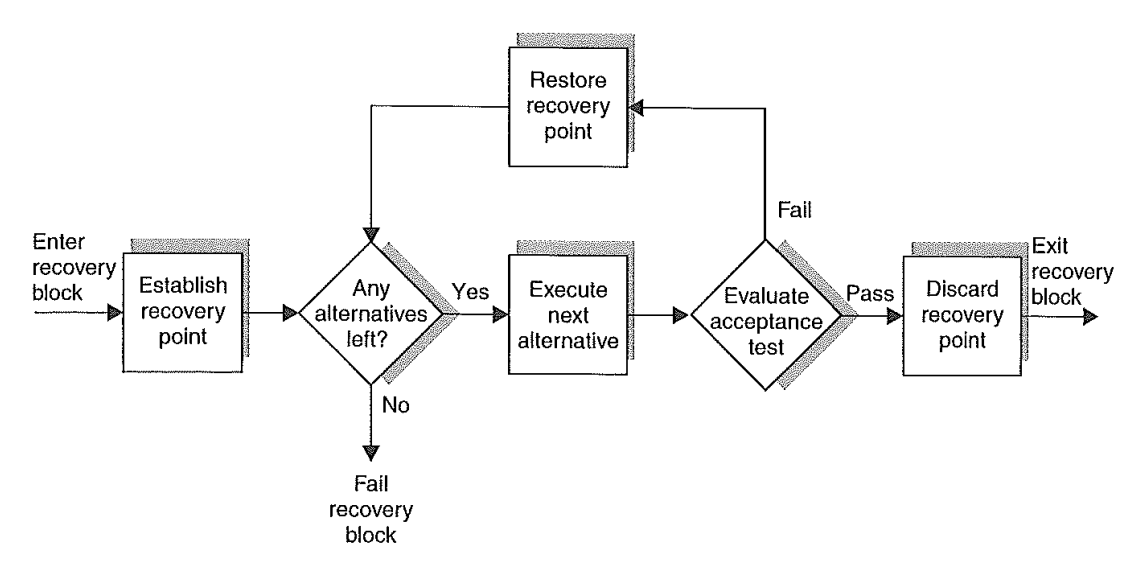
\includegraphics[width=0.8\textwidth]{recovery_block.png}
    \caption{Structure of a recovery block.}
    \label{fig:recovery_block}
\end{figure}

\subsection{Acceptance test}
The acceptance test provides an error detection mechanism, e.g. with invokations of \texttt{assert()}. There is always a trade-off between a comprehensive test and affecting the 'happy path' as little as possible. All the error detection techniques discussed in \Cref{sec:error_detection} can be used to create acceptance tests.

\section{Comparison between N-version programming and recovery blocks}
Brief comparison:
\begin{itemize}
    \item N-version is static, all versions run regardless of whether an error has occured or not. Recovery blocks are dynamic.
    \item N-version requires a driver process, while recovery blocks need an acceptance test. At run-time N-version requires N times the resources, since recovery blocks only run one code block at a time. However, establishing recovery points, and reverting to them is expensive.
    \item Both are prone to errors stemming from ambiguous specifications.
    \item Acceptance tests may be more flexibe than e.g. an inexact voting scheme. 
    \item The backward error recovery of recovery blocks cannot undo effects on the environment (not impossible to design a system that avoids this problem), whereas N-version requires everything to go through the driver before it can affect the outside world.
\end{itemize}

\section{Dynamic redundancy and exceptions}
\textbf{Exception} $:=$ the occurence of an error. Telling the 'invoker' about the error condition is called \textbf{raising} (or signaling or throwing) and exception, and the invoker then \textbf{handles} (or catches) the exception. 

Exceptions can be regarded as forward error recovery, as the state is not rolled back, but control is handed over to the exception handler (still, backward recovery can be implemented with exceptions). There is an example in B\&W that illustrates some of the controversy surrounding exceptions.
\newpage
\part{Fault model \& software fault masking}
Keywords from the part on basic fault tolerance are:
\begin{itemize}
    \item Acceptance tests
    \item Merging failure modes
    \item Redundancy
\end{itemize}
For a fault tolerant system we want the following (progressively better):
\begin{enumerate}
    \item Failfast (errors are detected immediately)
    \item Reliable (failfast + the system is repaired)
    \item Available (continuous operation)
\end{enumerate}
An overview of the process is:
\begin{enumerate}
    \item Find failure modes.
    \item Detect errors / simplify error model, inject errors for testing
    \item Error handling by redundancy $\rightarrow$ reliable and available module.
\end{enumerate}
On error injection:
\begin{enumerate}
    \item Simplify by merging failure modes.
    \item Inject failed acceptance tests.
\end{enumerate}
Examples for fault tolerant modules, three basic modules: storage, communication and processing.
\section{Storage}
Imagine an array of data. Assume unreliable read and write functions.
\subsection{Failure modes}
For writing we have:
\begin{itemize}
    \item Writes the wrong data
    \item Writes to the wrong place
    \item Does not write
    \item Fails
\end{itemize}
Likewise, for reading:
\begin{itemize}
    \item Give wrong data
    \item Give old data
    \item Give data from wrong place
    \item Fails
\end{itemize}

\subsection{Detection, merging of error modes and error injecction}
\begin{itemize}
    \item Detect by also writing address, checksum, versionID and statusbit to the buffer.
    \item Merging: All errors $\rightarrow$ Fail
    \item For error injection, spawn a thread that runs in parallel and flips status bits. This seems really smart!
\end{itemize}
\subsection{Handling with redundancy}
\begin{itemize}
    \item Keep several copies of the buffer, the one with the newest versionID is used (returned).
    \item Always write back when a reading error occurs (write a 'safe state'?).
    \item 
\end{itemize}
\section{Messages}
\subsection{Failure modes}
\begin{itemize}
    \item Lost
    \item Delayed
    \item Corrupted
    \item Duplicated
    \item Wrong recipient
\end{itemize}

\subsection{Detection, merging of error modes}
\begin{itemize}
    \item Session ID
    \item Checksum
    \item Ack (acknowledgement)
    \item Sequence numbers
    \item All errors $\rightarrow$ Lost message
\end{itemize}

\subsection{Handling with redundancy}
\begin{itemize}
    \item Timeout and retransmission
\end{itemize}

\section{Processes/calculations}
\textbf{Error mode:} Does not yield the next correct 'side effect'.\\
\textbf{Detect and merge:} All failed acceptance tests $\rightarrow$ STOP (failfast).\\
Three ways to handle with redundancy, described in the following subsections.

\subsection{Checkpoint-restart}
\begin{itemize}
    \item Write state to storage after each (successful) acceptance test, before each side effect.
    \item This yields error containment, but requires good acceptance tests.
\end{itemize}
\subsection{Process pairs}
\begin{itemize}
    \item Two processes; primary and backup (primary does the work).
    \item Backup takes over if (when) primary fails, and becomes new primary.
    \item Primary sends IAmAlive-messages and checkpoints to backup.
    \item NB! Because of resending this does not rely on safe communication. I.e. we get redundancy by resending, communication errors are masked out.
\end{itemize}

\subsection{Persistent processes}
\begin{itemize}
    \item Transactional infrastructure
    \item All calculations are transactions, i.e. atomic transformations from one consistent state to another.
    \item The processes are then 'stateless', all states are stored in a database.
    \item For such simple processes OS can take care of restart.
\end{itemize}
Note that reliable and available storage, communication and calculations are necessary to make this transactional infrastructure. Hence one often falls back to one of the first two options.

\newpage
\part{Transaction fundamentals}
Context and motivation for introducing transactions:
\begin{itemize}
    \item We need error handling and -containment for systems with multiple participants (threads, processes, distributed systems). These participants must often cooperate in the error handling.
    \item Transactions (and atomic actions) are techniques/frameworks that provide the means to do this. They fall under the category of dynamic SW redundancy.
    \item They contribute towards the desired 'error assessment and confinement' design, and help avoiding the 'domino effect'.
    \item A motivating example is a process control plant with many local controllers, supervisory tasks, monitoring, optimization, several modes of operation and high demands for safety.
\end{itemize}
From the learning goals, \textbf{eight design patterns}:
\begin{enumerate}
    \item Locking
    \item Two-phase commits
    \item Transaction manager (TM)
    \item Resource manager (RM)
    \item Log 
    \item Checkpoints
    \item Log manager
    \item Lock manager
\end{enumerate}
And some additional terms:
\begin{itemize}
    \item Optimistic concurrency control
    \item Two-phase commit optimization
    \item Heuristic transactions
    \item Interposition
\end{itemize}
\textbf{Atomic action:} Indivisible operation, either it happens or it does not at all.\newpage
\textbf{(Atomic) transaction:} 
\begin{itemize}
    \item All-or-nothing property to work conducted within its scope.
    \item Shared resources are protected.
\end{itemize}
ACID properties of transactions:
\begin{enumerate}
    \item Atomicity: The transaction either commits successfully or rolls back (aborts) completely at fail.
    \item Consistency: Preserve consistent state.
    \item Isolation: Intermediate states during a transaction are not visible to the outside. Further, transactions appear to be executing \emph{serially}, even when they are not.
    \item Durability: The effects of a commited transaction are never lost, i.e. they are stored in stable storage, such as disk.
\end{enumerate}
\textbf{Two-phase commits:}
Associated with each transaction is a coordinator C, that communicates with the participants. The message flow is as follows:
\begin{verbatim}
Coordinator                                         Participant
                              QUERY TO COMMIT
                -------------------------------->
                              VOTE YES/NO           prepare*/abort*
                <-------------------------------
commit*/abort*                COMMIT/ROLLBACK
                -------------------------------->
                              ACKNOWLEDGMENT        commit*/abort*
                <--------------------------------  
end
\end{verbatim}
The first phase is the commit request (or voting) phase, and includes lasts until the \texttt{VOTE YES/NO} arrow in the above diagram. The second phase is the commit phase, where the operation of each participant is either completed (if all votes were yes) or rolled back (if anyone voted no). Refer to \url{https://en.wikipedia.org/wiki/Two-phase_commit_protocol} for more on the algortihm.

A disadvantage with two-phase commits is that the protocol is blocking. Participants will block after they have voted, awaiting a commit or rollback message. If the coordinator fails, they will never receive either.


% Next up: Read about transactions and atomic actions, etc. Use pseucocode actively. Read about code quality. Start doing exams.  




\newpage
\part{Shared variable synchronization}
\section{Semaphores}
A \textbf{semaphore} is like an integer, with three key differences:
\begin{enumerate}
    \item It can be initialized to any value, but after that only incremented or decremented (its value cannot be read).
    \item When the semaphore is decremented by a thread, and the result is negative, the thread blocks.
    \item When the semaphore is incremented by a thread, one waiting thread gets unblocked (if any).
\end{enumerate} 
Things to note:
\begin{itemize}
    \item After one thread increments the semaphore, and another is woken, they run concurrently.
    \item A positive value represents the number of threads that can decrement without blocking.
    \item A negative number represents the number threads that have blocked and are waiting.
\end{itemize}
The basic syntax used is:
\begin{itemize}
    \item \texttt{sem = Semaphore(1)} to create a new semaphore with the given initial value.
    \item \texttt{sem.signal()} to increment the semaphore (and wake a waiting thread).
    \item \texttt{sem.wait()} to decrement the semaphore (and block if the result is negative).
\end{itemize}
In the classical example of incrementing/decrementing \texttt{int i}, \texttt{i}'s value must be set pretty high to see synchronization errors. The reason for this is that context switching (switching between threads and saving states) does not happen until a certain time passes. For small \texttt{i}, one thread will typically finish before the second gets a chance to start.

\section{Standard problems}
A (data) \textbf{race condition} is a fault in the design of the interaction between two threads, which leads to the result being highly dependent on the sequence and timing of access to shared variables.

A \textbf{livelock} occurs when a thread gets stuck in e.g. a busy-waiting loop (more generally; a subset of the possible states), and is unable to proceed.

A \textbf{deadlock} occurs when the system is stuck in a circular wait, with no threads being able to proceed. 

\textbf{Starvation} happens when a thread is unable to gain access to a resource it requires, because other threads keep getting it first. Can be caused by an 'unfair' scheduler.

\section{Monitors}
What is bad with semaphores?
\begin{itemize}
    \item Forgetting a wait can lead to multplie threads running concurrently in a \textbf{critical region} (a section of code that should always be executed under mutual exclusion).
    \item Forgetting a signal can lead to a deadlock.
    \item The code is distributed all over the system, making maintenance hard.
\end{itemize}

\subsection{Critical regions}
\begin{itemize}
    \item Critical regions but the responsibility for mutual exclusion on the compiler, instead of the programmer. Critical regions of the same name mutually exclude.
    \item In \textbf{conditional critical regions}, the thread must wait for the mutex lock \emph{and} check a boolean condition before it can proceed. A \textbf{guard} is a more sophisticated form of this boolean condition, which instead runs a test (procedure) that opens or closes for execution.
\end{itemize}
Limitations
\begin{itemize}
    \item (Conditional) critical regions are still distributed throughout the program.
\end{itemize}

\subsection{Monitors}
\begin{itemize}
    \item A collection of local variables and procedures (basically a module), with a mutex that only allows one thread at a time to access its methods and variables.
    \item Pro: All code that accesses the shared data is localized.
    \item Has \textbf{condition variables} (queues of threads waiting for some condition to be true) with operations \texttt{suspend} and \texttt{resume} to block and unblock threads.
    \item \texttt{suspend} releases the monitor lock.
    \item The operations are safe, because they can only be accessed/called from inside the monitor.
\end{itemize}
Cons
\begin{itemize}
    \item Suspending in a nested call does not release the outer lock. Ex. a procedure in monitor A calls a procedure in monitor B, which contains a \texttt{suspend} statement. This makes it infeasible to build supermodules from submodules (that are monitors). 
    \item The possibility for deadlocks and data races still exists.
    \item Does not provide other synchronization than condition variables.
\end{itemize}

\section{Synchronization mechanisms in POSIX, Java and Ada}
\subsection{Java}
The \texttt{synchronized} keyword is used to make methods thread-safe. Consider the following class:
\begin{minted}{java}
    public class MyClass {
        private int i;

        public MyClass(int initValue) {
            i = initValue;
        }

        public synchronized void increment() {
            i++;
        }
    }
\end{minted}
When thread A is executing \texttt{increment()}, all other threads that (wish to) invoke synchronized methods for the same \texttt{MyClass}-object block (suspend) until thread A releases the monitor lock.

\texttt{wait()} is used to suspend the current thread, like this:
\begin{minted}{java}
    public synchronized void conditionalIncrement() {
        while(i < 3) wait();
        i++;
    }
\end{minted}
Note that since the method is \texttt{synchronized}, thread A must hold the monitor lock before it can invoke it. When it calls \texttt{wait()}, it releases the lock and suspends execution. It will be woken up at some time after the following procedure has run:
\begin{minted}{java}
    public synchronized void importantChange() {
        i = 3;
        notifyAll();
    }
\end{minted} 
All threads waiting on the lock are notified when \texttt{notifyAll()} is called.

\subsection{Ada}
Ada offers monitors as \emph{protected modules}. A protected module can be either a single protected object or a protected type, which can contain many objects. 

\newpage
\part{Scheduling}
Concurrent programs exhibit non-determinism, and a real-time system needs to restrict this non-determinism through scheduling. A scheduling scheme provides two key features:
\begin{enumerate}
    \item An algorithm for ordering the use of system (CPU) resources.
    \item A way to predict the worst-case behavior of the system when the scheduling algorithm is applied.
\end{enumerate}  
There are \textbf{static} (prediction only before execution) and \textbf{dynamic} (run-time decisions are used) schemes. Focus for us: static schemes, specifically preemptive priority-based schemes on a single-processor system. The task with the highest priority will always run, unless it is suspended or delayed for some reason. The two features above can be re-stated as:
\begin{enumerate}
    \item Priority assignment algorithm
    \item Schedulability test
\end{enumerate}

\subsection{Non-preemptive scheduling (cyclic executive)}
What is non-preemptive scheduling?
\begin{itemize}
    \item Fixed set of tasks with fixed periods.
    \item Consists of a table of procedure calls, the major cycle, comprised of smaller minor cycles with fixed duration.
    \item At run-time, no tasks run concurrently, therefore mutual exclusion is guaranteed (we don't need e.g. semaphores).
    \item All task periods must be a multiple of the minor cycle period (obvious drawback).
\end{itemize}
What are some of its drawbacks?
\begin{itemize}
    \item Difficult to incorporate sporadic tasks.
    \item Difficult to construct.
    \item Difficult to incorporate tasks with long periods
    \item 'Large' tasks will need to be split up into several procedures, which may hurt the quality of the code, and make it more error-prone.
\end{itemize}

\subsection{Task-based scheduling}


\end{document}
